% Manuscript in a neutral single-column layout (compiles with any TeX Live).
% For the Springer Nature template use main_sn.tex (needs sn-jnl.cls from Springer).
\documentclass[11pt,a4paper]{article}
\usepackage[T1]{fontenc}
\usepackage[utf8]{inputenc}
\IfFileExists{lmodern.sty}{\usepackage{lmodern}}{}
\usepackage[margin=25mm]{geometry}
\usepackage{amsmath,amssymb}
\usepackage{graphicx}
\usepackage{booktabs}
\usepackage{amssymb}
\usepackage{tikz}
\usetikzlibrary{positioning,shapes.geometric,arrows.meta,calc}
\usepackage[numbers,sort&compress]{natbib}
\usepackage{lineno}
\usepackage[hidelinks]{hyperref}
\usepackage{setspace}
\setstretch{1.15}
\linenumbers

\title{Gait-Phase-Aware Command Timing for Decentralized Quadruped Swarms}
\author{Bishwaswarup Nayak\\[2pt]
  \small Indian Institute of Science, Bengaluru, India\\
  \small \texttt{bishwaswarup@iisc.ac.in} (corresponding author)}
\date{}

\begin{document}
\maketitle

\begin{abstract}
Multi-robot collision avoidance treats each robot as a point that can change velocity at any instant. A
trotting quadruped cannot: how well it absorbs a change of commanded velocity depends on where in the gait
cycle the change arrives. We measure this dependence for a B\'ezier-curve trot controller on a simulated
Unitree Go1 and use it in a decentralized swarm. The phase-aware layer solves reciprocal collision avoidance
(ORCA) one gait period ahead, releases each new velocity command at the gait phase our capability map
predicts is least destabilizing, and shapes it with a gait-aware slew limiter; urgent conflicts bypass the
timing. In MuJoCo, across 4 to 32 robots in antipodal swaps, pillar fields, a narrow gate and a 53\,m obstacle
course, the full system is compared with the same stack without timing (790 runs, paired by seed,
Holm-corrected). In crowded and obstructed scenarios it cuts urgent avoidance events by 22--39\% and
99th-percentile body tilt by 19--24\%, increases the closest robot--robot distance in formations by 2--5\,cm,
and had no falls in any run. Prediction without phase timing gives no consistent benefit, so the timing is the
active ingredient. In sparse traffic (four robots) the method costs more than it saves.

\end{abstract}

\noindent\textbf{Keywords:} legged robots $\cdot$ multi-robot systems $\cdot$ collision avoidance $\cdot$
gait phase $\cdot$ quadruped swarms $\cdot$ ORCA

% ---------------------------------------------------------------------------
% Shared body: \input by main.tex (article class, compiles anywhere) and by
% main_sn.tex (Springer Nature sn-jnl class).
% ---------------------------------------------------------------------------

\section{Introduction}\label{sec:intro}

Decentralized collision avoidance methods such as reciprocal velocity obstacles and ORCA
\cite{vandenberg2008rvo,vandenberg2011orca} give each robot a new velocity every control tick. They assume
that the platform can follow that velocity, possibly subject to an acceleration limit. Wheeled robots and
multirotors come close to that assumption. A trotting quadruped does not: its body is supported by two
diagonal feet at a time, the support line rotates during each stance, and a velocity change that arrives
at the wrong moment produces a large body tilt or a stumble.

That a legged gait responds to a disturbance differently at different phases is well known in
single-robot locomotion: push recovery, capture-point and step-timing methods all exploit it
\cite{pratt2006capture,khadiv2016step,chen2022capturability,hobbelen2007gsn}. What has not been studied,
to our knowledge, is the consequence for multi-robot navigation. A swarm layer that issues frequent
avoidance commands is a source of disturbances to every robot's gait. Formation and swarm controllers for
quadrupeds \cite{zhan2025safe,noren2026role} shape \emph{what} each robot is commanded, but not \emph{when}
within the gait the command is delivered.

This paper asks one question: does timing the swarm layer's velocity changes to the gait phase make a
quadruped swarm safer, and at what cost? We answer it in simulation with a fully open stack and paired
statistics. Our contributions are:
\begin{enumerate}
  \item A measurement of phase-dependent fragility for a B\'ezier trot on a Unitree Go1 model: a pilot
    experiment, a capability map over phase, direction and size of a command change (held-out
    $R^2$ 0.94--0.98, against 0.70--0.87 without phase), and a push-impulse envelope in which knowing the
    phase raises the tolerable impulse by a factor of 1.33--1.44.
  \item A phase-aware command layer: a commander that releases each velocity change at the predicted best
    phase within a deadline, and a gait-aware slew limiter that shapes the change by phase.
  \item A predictive ORCA layer that plans one gait period ahead, so that the commander has time to wait
    for a good phase, with an urgent bypass when the time to collision is short.
  \item An ablation and scaling study over 4--32 robots, a gate, pillar fields and a 53\,m obstacle course
    (790 runs in the final configuration, paired by seed, Holm-corrected), including negative results:
    where the method does not help, and a robustness fix we tried and rejected.
\end{enumerate}

\section{Related work}\label{sec:related}

\paragraph{Reciprocal collision avoidance.} Velocity obstacles and their reciprocal forms
\cite{vandenberg2008rvo,vandenberg2011orca} are the standard decentralized method for crowds of robots;
ORCA reduces each control tick to a small linear program. Extensions add platform limits:
acceleration-velocity obstacles bound the acceleration \cite{vandenberg2011avo}, and NH-ORCA bounds the
tracking error of non-holonomic robots \cite{alonsomora2013nhorca}. All of these model the platform's
limits as constant in time. We keep ORCA unchanged and instead model a limit that varies periodically with
the gait.

\paragraph{Multi-quadruped formation and navigation.} Recent work on quadruped teams uses distributed model
predictive control with control barrier functions \cite{zhan2025safe} or leader--follower formations with
path planning \cite{noren2026role}. These treat each quadruped as a velocity-controlled point and rely on
the locomotion controller to follow the commands. The phase-aware layer proposed here is complementary: it
can sit between any such planner and the locomotion controller.

\paragraph{Phase-dependent response of legged gaits.} The capture point \cite{pratt2006capture}, step-timing
adaptation \cite{khadiv2016step} and switched-system capturability for quadrupeds
\cite{chen2022capturability} all show that what a legged robot can recover from depends on its state
within the step, and gait-sensitivity analysis \cite{hobbelen2007gsn} measures how disturbances propagate
through a limit cycle. These results are used to choose footholds and step times for one robot. We use the
same fact one level up: to choose \emph{when} the navigation layer changes its command.

\paragraph{Command shaping for legged robots.} Velocity commands to legged controllers are commonly
rate-limited, and learned controllers are trained on curricula of command changes. A recent example
schedules commands by the robot's current velocity to reach high speed \cite{tao2026speed}. To our
knowledge, no prior work schedules navigation commands by gait phase.

\section{The low-level controller and its phase-dependent fragility}\label{sec:controller}

\paragraph{Controller.} Each robot runs the same open-source trot controller. The feet follow a 12-point
B\'ezier swing curve \cite{hyun2014cheetah,rahme2020spotmini} in a diagonal trot (period 0.36\,s, duty factor
0.5, swing clearance 0.07\,m, hip-to-foot height 0.27\,m). A PI loop on body velocity ($k_i = 1.5$) removes
steady drift, Raibert foot placement \cite{raibert1986legged} (gain 0.1) corrects velocity errors, and joint
targets go to the position actuators of the MuJoCo Menagerie Go1 model
\cite{todorov2012mujoco,zakka2022menagerie}. A slew limiter bounds the rate of change of the command at
$(1.5\,\mathrm{m/s^2}, 1.0\,\mathrm{m/s^2}, 3.0\,\mathrm{rad/s^2})$ for $(v_x, v_y, \omega_z)$. The
controller tracks commands to within about 0.02\,m/s, survives 4\,min of random command changes without a
fall, and walks at heights from 0.16\,m to 0.34\,m.

\paragraph{Stability.} Treating one gait period as a stroboscopic Poincar\'e map, the largest Floquet
multiplier is 0.42--0.59 for the full controller and 0.73--0.87 open loop, so the gait is orbitally stable
over the commanded speed range. Stability of the cycle does not say how a single command change is
absorbed, which depends on when it arrives.

\paragraph{Why the phase matters.} In a trot the body is supported by one diagonal pair at a time: front-right
with rear-left, then front-left with rear-right, at roughly $-34^\circ$ and $+34^\circ$ to the heading for the
Go1's geometry. Within one stance the effective support axis rotates from about $+25^\circ$ to $+65^\circ$ as
the body moves over the feet. A change of commanded velocity that pushes the body across the current support
axis is resisted by the stance legs; one that pushes along it tips the body about that axis. The same change
therefore produces different tilt at different phases, and by the mirror symmetry of the trot the pattern
repeats every half period with the lateral direction flipped.

\paragraph{Measured fragility.} A pilot experiment applied command steps and body pushes at controlled phases.
Phase had a large effect: in 27 of 64 push conditions, whether the robot recovered depended on the phase
alone. From these data we built a capability map: a lookup table, periodic in phase and symmetrized, that
predicts peak tilt and fall risk for a command change of a given direction and size at a given phase
(Fig.~\ref{fig:phase}a). On held-out trials it explains 94--98\% of the variance, against 70--87\% for the
same model without phase. A push-impulse envelope found by bisection (Fig.~\ref{fig:phase}b) agrees with the
pilot in 98.6\% of cases, and knowing the phase raises the impulse the robot tolerates by a factor of
1.33--1.44.

\begin{figure*}[t]
  \centering
  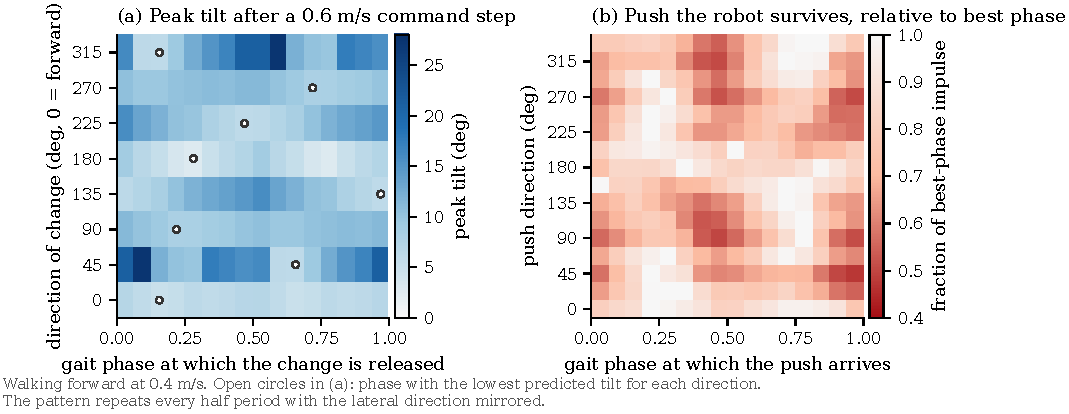
\includegraphics[width=\textwidth]{figures/fig2_phase.pdf}
  \caption{Phase dependence of the trot controller while walking forward at 0.4\,m/s. (a) Peak body tilt
  after a 0.6\,m/s step in commanded velocity, by direction of the change and the gait phase at which it is
  released; open circles mark the best phase for each direction. (b) Largest push impulse the robot survives,
  as a fraction of the value at its best phase for that direction.}
  \label{fig:phase}
\end{figure*}

\paragraph{What this means for a swarm.} In isolated step tests, releasing a command at the best phase
strictly dominated the slew limiter alone. In a stream of swarm commands, however, timing alone did not work:
only 0--2\% of the commands resembled the settled single steps the map was measured on, and about half were
urgent, leaving no time to wait for a good phase. Section~\ref{sec:method} is designed around that finding:
the swarm layer must look ahead so that most changes are known before they are needed.

\section{Method}\label{sec:method}

Every robot runs the same four-stage stack at 10\,Hz (Fig.~\ref{fig:stack}), with no central planner and no
communication beyond the neighbour positions and velocities that ORCA needs. A safety layer that is
identical in every configuration, the baseline included, wraps the stack.

\begin{figure}[t]
  \centering
  \resizebox{\columnwidth}{!}{%
  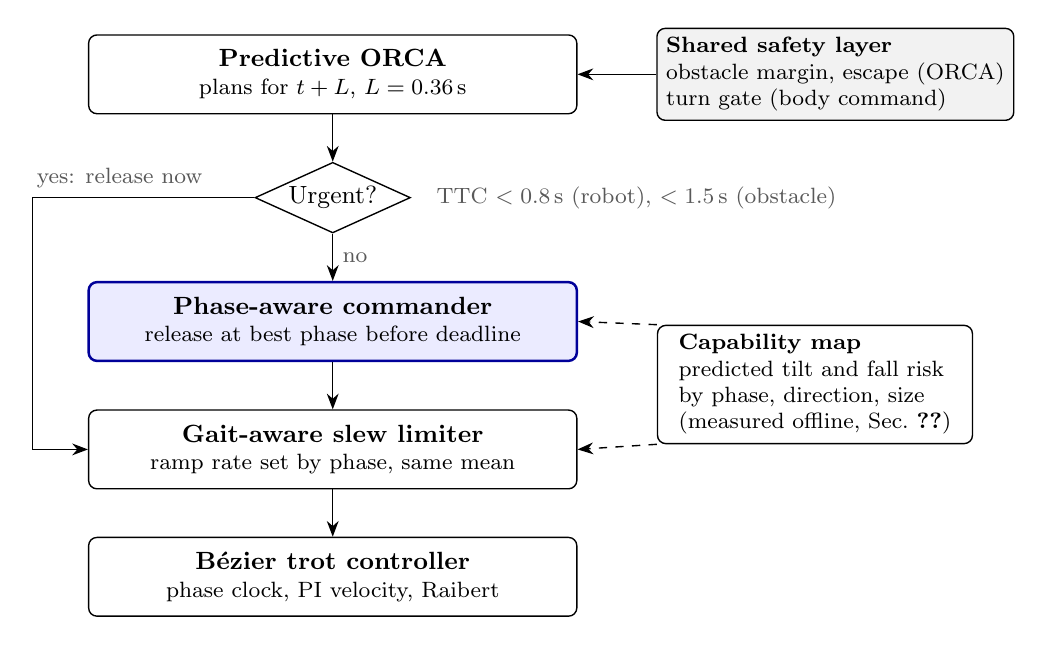
\begin{tikzpicture}[
      node distance=6mm and 10mm, font=\small,
      box/.style={draw, rounded corners=3pt, align=center, minimum width=62mm, minimum height=10mm, line width=0.5pt},
      main/.style={box, draw=blue!60!black, fill=blue!8, line width=0.9pt},
      side/.style={draw, rounded corners=3pt, align=left, minimum width=40mm, font=\footnotesize, line width=0.5pt},
      dec/.style={draw, diamond, aspect=2.2, inner sep=1pt, align=center, line width=0.5pt},
      arr/.style={-{Stealth[length=2mm]}, line width=0.5pt},
      note/.style={font=\footnotesize, text=black!65}]
    \node[box] (orca) {\textbf{Predictive ORCA}\\[-1pt]{\footnotesize plans for $t+L$, $L = 0.36$\,s}};
    \node[dec, below=of orca] (urg) {Urgent?};
    \node[main, below=of urg] (cmd) {\textbf{Phase-aware commander}\\[-1pt]{\footnotesize release at best phase before deadline}};
    \node[box, below=of cmd] (lim) {\textbf{Gait-aware slew limiter}\\[-1pt]{\footnotesize ramp rate set by phase, same mean}};
    \node[box, below=of lim] (trot) {\textbf{B\'ezier trot controller}\\[-1pt]{\footnotesize phase clock, PI velocity, Raibert}};
    \node[side, right=of orca, fill=black!5] (safe) {\textbf{Shared safety layer}\\obstacle margin, escape (ORCA)\\turn gate (body command)};
    \node[side, right=of cmd, yshift=-8mm] (map) {\textbf{Capability map}\\predicted tilt and fall risk\\by phase, direction, size\\(measured offline, Sec.~\ref{sec:controller})};
    \draw[arr] (orca) -- (urg);
    \draw[arr] (urg) -- node[right, note] {no} (cmd);
    \draw[arr] (cmd) -- (lim);
    \draw[arr] (lim) -- (trot);
    \coordinate (bx) at ($(cmd.west)+(-7mm,0)$);
    \draw[arr] (urg.west) -- (urg.west -| bx) node[above, note, pos=0.5, xshift=-3mm] {yes: release now} -- (bx |- lim.west) -- (lim.west);
    \draw[arr] (safe) -- (orca);
    \draw[arr, dashed] (map.north west) -- (cmd.east);
    \draw[arr, dashed] (map.south west) -- (lim.east);
    \node[note, right=2mm of urg] {TTC $<0.8$\,s (robot), $<1.5$\,s (obstacle)};
  \end{tikzpicture}}
  \caption{Per-robot stack. ORCA plans one gait period ahead; non-urgent changes wait in the commander for the
  phase the capability map predicts is safest, urgent ones go straight to the limiter. The safety layer is
  the same in every configuration.}
  \label{fig:stack}
\end{figure}

\paragraph{Predictive swarm layer.} Each robot is a disc of radius 0.38\,m with maximum speed 0.6\,m/s.
Rather than solving ORCA for the present, the robot solves it for the situation one lookahead $L$ ahead
($L = 0.36$\,s, one gait period). Its own position is extrapolated with the command it is currently executing,
and its neighbours with their measured velocities. The result is the velocity the robot will need at time
$t + L$, so it can be requested with a deadline of $L$. If the current command would collide within 0.8\,s
with a robot, or within 1.5\,s with a static obstacle, the request is urgent: ORCA is solved for the present
and the command is released at once. A $15^\circ$ keep-right bias breaks symmetric deadlocks.

\paragraph{Phase-aware commander.} A request whose change from the current command exceeds 0.15\,m/s
(or 0.3\,rad/s) is a manoeuvre. For each manoeuvre the commander queries the capability map for every gait
phase reachable before the deadline (at most 0.5\,s) and releases the command at the phase with the lowest
predicted cost, namely peak tilt plus a weight of 50 on the predicted fall probability. Smaller changes,
urgent requests and changes outside the map's domain are released at once. A new request similar to a pending
one keeps the pending release time, so the timing is not reset every tick.

\paragraph{Gait-aware slew limiter.} Once released, a change is applied through a slew limiter whose rate
depends on phase. The limiter is built from the capability map: it ramps faster in phases where the map
predicts little tilt for the current direction of change and slower where it predicts a lot. Its rate is
scaled so that its mean over one period equals that of the uniform limiter, so it does not gain speed by
being more aggressive on average.

\paragraph{Formation and queueing.} Formations follow a reference point with slot offsets that shrink
laterally when obstacles are close ahead. In bottlenecks, the robot further back takes 90\% of the avoidance
responsibility in ORCA and the robot in front 10\%, so that robots queue instead of shouldering through.

\paragraph{Shared safety layer.} In every configuration, ORCA sees static obstacles inflated by 0.1\,m with a
2\,s horizon. Body commands are clipped to the range in which the gait was stress-tested
($|\omega_z| \le 1.0$\,rad/s, $|v_y| \le 0.3$\,m/s), and forward speed is scaled from 100\% to 30\% as the
heading error grows from $30^\circ$ to $90^\circ$, so a robot turns before it walks. If ORCA returns less than
0.05\,m/s for more than 1\,s while the robot wants to move, the preferred velocity is turned $75^\circ$
towards the formation reference for 2\,s, and to the other side if the robot is still stuck. Each of these
was added after a failure found in the experiments; Section~\ref{sec:discussion} reports one further fix that
we tried and rejected.

\section{Experimental setup}\label{sec:setup}

All experiments run in MuJoCo \cite{todorov2012mujoco} with $N$ copies of the Menagerie Go1 model
\cite{zakka2022menagerie} in one scene (foot friction 0.9). The swarm layer runs at 10\,Hz and the gait
controller at the physics rate. Each seed perturbs every start position by 5\,cm (standard deviation) and
gives every robot a random initial gait phase, so robots are never phase-locked. Table~\ref{tab:scenarios}
lists the scenarios and Table~\ref{tab:configs} the configurations.

\begin{table*}[t]
  \centering
  \caption{Scenarios.}
  \label{tab:scenarios}
  \small
  \begin{tabular}{@{}l p{24mm} p{62mm} p{38mm}@{}}
    \toprule
    Scenario & Robots & Layout & Tests \\
    \midrule
    Swap & 4 / 8 / 16 / 32 & On a circle of radius 2.5 / 4 / 6 / 9\,m; each robot walks to the opposite point & Crossing traffic; density grows with $N$ \\
    Pillars & 9 ($3\times3$, 1.4\,m spacing) & Formation travels 14\,m at 0.35\,m/s through 5 pillars ($r = 0.3$\,m) & Formation through clutter \\
    Gate & 6 ($2\times3$) & Wall with a 1.9\,m opening & Bottleneck: the team narrows and queues \\
    Pillars & 16 ($4\times4$) & 18\,m through 9 pillars & Dense formation through clutter \\
    Course & 1 and 6 & 53\,m path at 0.45\,m/s: pole slalom, 1.9\,m gate, chicane, two obstacles moving across the path (0.4\,m/s), 7 pillars & All of the above in sequence \\
    \bottomrule
  \end{tabular}
\end{table*}

\begin{table}[t]
  \centering
  \caption{Configurations. All share the safety layer of Section~\ref{sec:method}.}
  \label{tab:configs}
  \small
  \begin{tabular}{@{}lcccc@{}}
    \toprule
    Configuration & Prediction & Timing & Limiter & Queue \\
    \midrule
    Baseline (reactive)      & -- & -- & -- & -- \\
    Queueing only            & -- & -- & -- & \checkmark \\
    Prediction only          & \checkmark & -- & -- & -- \\
    Prediction + timing      & \checkmark & \checkmark & -- & -- \\
    \quad + gait-aware limiter & \checkmark & \checkmark & \checkmark & -- \\
    Full system              & \checkmark & \checkmark & \checkmark & \checkmark \\
    \bottomrule
  \end{tabular}
\end{table}

The main suite runs all six configurations on the 4- and 8-robot swaps, the 9-robot pillar field and the gate
with 20 seeds (480 runs). The scaling suite runs the baseline, prediction only (with queueing) and the full
system on the 16- and 32-robot swaps and the 16-robot pillar field with 10 seeds (90 runs). The lookahead suite
varies $L \in \{0.18, 0.36, 0.54, 0.72\}$\,s on the 8-robot swap and the gate (10 seeds, 100 runs). The
course runs three configurations for teams of 1 and 6 robots with 20 seeds (120 runs).

\paragraph{Metrics.} Three metrics are fixed in advance as primary: urgent avoidance events per robot-minute
(how often a robot had to change course with less than 0.8\,s to spare), the 99th-percentile body tilt over
the run, and the closest robot--robot distance. We also report falls (trunk below 0.15\,m or tilted more than
$60^\circ$), runs not finished within the time limit, contacts and completion time.

\paragraph{Statistics.} Each configuration is compared with the baseline on the same seed. For each metric we
take the per-seed difference and test it with a two-sided sign-flip permutation test (exact for up to 16
seeds, 20{,}000 random sign patterns otherwise), with 95\% bootstrap confidence intervals. The 21 primary
tests (7 scenarios $\times$ 3 metrics, full system against baseline) are corrected together with the Holm
method. With 10 seeds the smallest attainable corrected $p$-value is about 0.02, which limits what the scaling
suite can show.

\section{Results}\label{sec:results}

The full system reduces urgent events and tilt wherever robots crowd or obstacles force manoeuvres, and does
no good in sparse traffic (Fig.~\ref{fig:primary}, Table~\ref{tab:primary}). Of the 21 primary tests, 15 are
significant after Holm correction: 13 favour the full system and 2, both in the 4-robot swap, favour the
baseline.

\begin{figure*}[t]
  \centering
  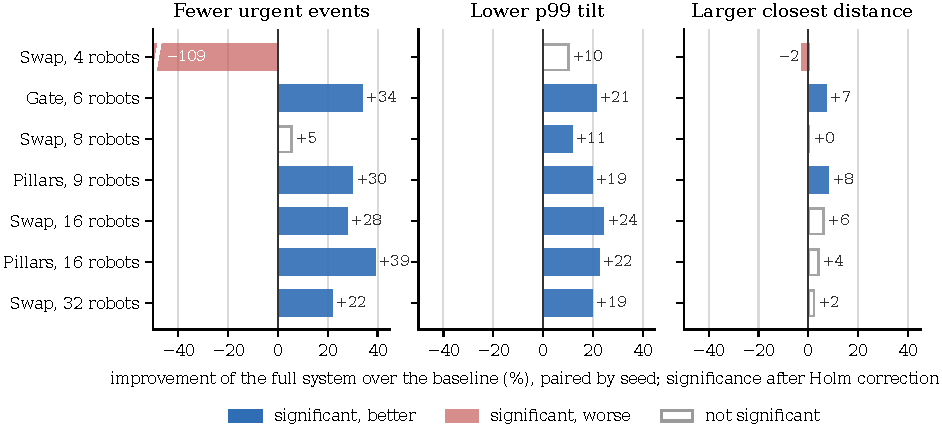
\includegraphics[width=\textwidth]{figures/fig3_primary.pdf}
  \caption{Improvement of the full system over the baseline on the three primary metrics. Filled bars are
  significant after Holm correction over all 21 tests. The 4-robot swap bar for urgent events is cut at
  $-50\%$ (true value $-109\%$).}
  \label{fig:primary}
\end{figure*}

\begin{table*}[t]
  \centering
  \caption{Primary metrics, baseline (B) against full system (F), means over seeds.
  $^{*}$\,$p<0.05$, $^{**}$\,$p<0.01$ after Holm correction over all 21 tests.}
  \label{tab:primary}
  \small
  \begin{tabular}{@{}lrr rrr rrr rrr@{}}
    \toprule
     & & & \multicolumn{3}{c}{Urgent events / robot-min} & \multicolumn{3}{c}{p99 tilt (deg)} & \multicolumn{3}{c}{Closest distance (m)} \\
    \cmidrule(lr){4-6}\cmidrule(lr){7-9}\cmidrule(l){10-12}
    Scenario & $N$ & Seeds & B & F & Change & B & F & Change & B & F & Change \\
    \midrule
Swap & 4 & 20 & 5.2 & 10.9 & +109\%$^{**}$ & 5.90 & 5.30 & $-$10\% & 0.744 & 0.727 & $-$2\%$^{**}$ \\
Gate & 6 & 20 & 24.4 & 16.2 & $-$34\%$^{**}$ & 5.84 & 4.62 & $-$21\%$^{**}$ & 0.661 & 0.707 & +7\%$^{**}$ \\
Swap & 8 & 20 & 29.6 & 28.0 & $-$5\% & 7.37 & 6.54 & $-$11\%$^{**}$ & 0.626 & 0.628 & +0\% \\
Pillars & 9 & 20 & 40.4 & 28.4 & $-$30\%$^{**}$ & 7.14 & 5.76 & $-$19\%$^{**}$ & 0.604 & 0.651 & +8\%$^{**}$ \\
Swap & 16 & 10 & 54.1 & 39.2 & $-$28\%$^{*}$ & 8.51 & 6.46 & $-$24\%$^{*}$ & 0.600 & 0.637 & +6\% \\
Pillars & 16 & 10 & 42.0 & 25.7 & $-$39\%$^{*}$ & 7.22 & 5.62 & $-$22\%$^{*}$ & 0.593 & 0.617 & +4\% \\
Swap & 32 & 10 & 64.5 & 50.6 & $-$22\%$^{*}$ & 8.39 & 6.76 & $-$19\%$^{*}$ & 0.566 & 0.578 & +2\% \\
    \bottomrule
  \end{tabular}
\end{table*}

\paragraph{Which component does the work.} Prediction alone does not help (Fig.~\ref{fig:ablation}). Against
the baseline it changes urgent events by $+6\%$ in the 8-robot swap and $+3\%$ in the pillar field, and raises
99th-percentile tilt by 20\% in the 4-robot swap. Adding phase timing produces most of the gain: urgent events
fall by 15--16\% and tilt by 12--16\% in the 8-robot swap, the pillars and the gate. The gait-aware limiter adds
further tilt reduction at the gate ($-15\%$ instead of $-12\%$) but almost none elsewhere. Queueing matters in
obstructed formations, where it doubles the reduction in urgent events (pillars $-30\%$ instead of $-18\%$,
gate $-34\%$ instead of $-14\%$) and widens the closest distance by 7--8\%. Phase timing is therefore the
active ingredient, and queueing is a useful complement only where robots must pass through gaps.

\begin{figure*}[t]
  \centering
  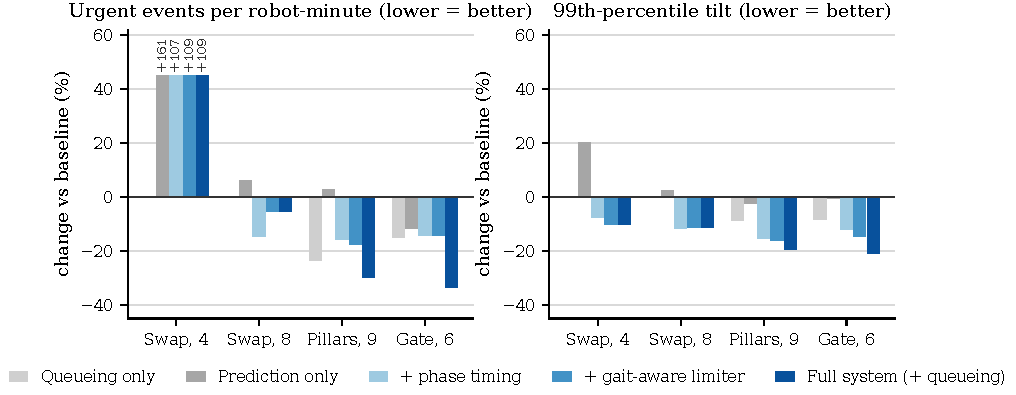
\includegraphics[width=\textwidth]{figures/fig4_ablation.pdf}
  \caption{Ablation on the main suite (20 seeds). Change relative to the reactive baseline as components are
  added; lower is better. Prediction alone does not help; phase timing produces most of the gain.}
  \label{fig:ablation}
\end{figure*}

\paragraph{Scaling.} The benefit holds as the team grows. With 16 robots in a swap the full system cuts urgent
events by 28\% and tilt by 24\%; with 32 robots, by 22\% and 19\%; with 16 robots in a formation through
pillars, by 39\% and 22\%. The gain in closest distance shrinks at 32 robots ($+2\%$, not significant), where
the swarm is near its packing limit.

\paragraph{Cost.} Waiting for a good phase costs time when there is nothing to avoid. In the 4-robot swap the
full system is 6.8\% slower, has twice the urgent events of the baseline (5.2 against 10.9 per robot-minute)
and a 2\% smaller closest distance. In the 8-robot swap it is 2.7\% slower; at the gate the completion time is
unchanged.

\paragraph{Lookahead.} Looking further ahead lets more changes be planned (Fig.~\ref{fig:lookahead}): the share
of manoeuvres that are urgent falls from 56\% (baseline) to 43\%, 41\%, 25\% and 22\% for $L$ = 0.18, 0.36,
0.54 and 0.72\,s in the 8-robot swap. But the number of command changes per robot-minute doubles from 54 to
112, because predictions made further ahead are revised more often. Tilt is reduced about equally at every
$L$. One gait period (0.36\,s) is the setting we use; 0.54\,s is slightly better at the gate but costs much
more command churn in swaps.

\begin{figure*}[t]
  \centering
  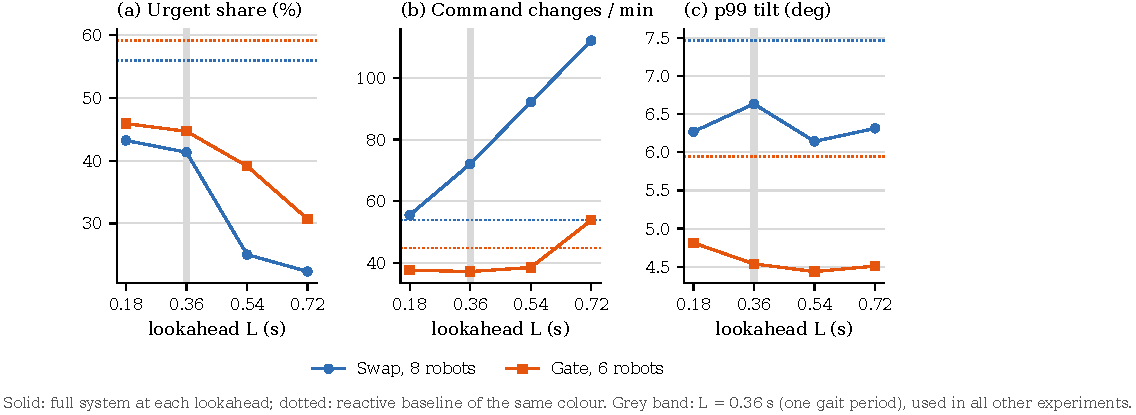
\includegraphics[width=\textwidth]{figures/fig5_lookahead.pdf}
  \caption{Effect of the lookahead $L$ (10 seeds). Longer lookahead makes fewer manoeuvres urgent (a) but
  increases command churn (b); tilt is reduced about equally at every $L$ (c).}
  \label{fig:lookahead}
\end{figure*}

\paragraph{Obstacle course.} For the team of six, the full system lowered 99th-percentile tilt from
$7.95^\circ$ to $6.68^\circ$ ($-16\%$), the worst tilt over 20 runs from $18.3^\circ$ to $13.7^\circ$, urgent
events by 14\% and robot--robot contacts from 0.25 to 0.05 per run, at the same completion time (129\,s).
Fig.~\ref{fig:course} shows one seed. One of its 20 runs did not finish in time; the baseline had one fall. For
a single robot the three configurations are nearly identical (tilt $4.7$--$4.9^\circ$), and prediction raised
urgent events (7.4 to 10.4 per minute), consistent with the 4-robot swap.

\begin{figure*}[t]
  \centering
  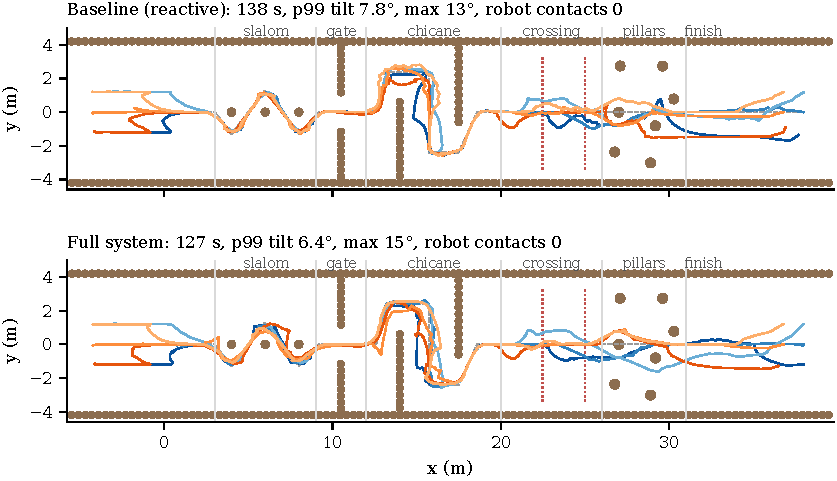
\includegraphics[width=\textwidth]{figures/fig6_course.pdf}
  \caption{Paths of a six-robot team on the obstacle course (seed 0) for the baseline (top) and the full system
  (bottom). Dotted red lines: tracks of the two moving obstacles; dashed grey line: reference path.}
  \label{fig:course}
\end{figure*}

\paragraph{Safety totals.} Across all 230 full-system runs in the final configuration there were no falls; the
baseline fell twice in 170 runs (once in the 16-robot pillar field and once on the course). Runs that did not
finish in time were rare in every configuration: one for the full system (course), one for queueing only and
two for prediction only.

\section{Discussion and limitations}\label{sec:discussion}

\paragraph{When it helps.} Phase timing pays off when a robot has many manoeuvres to make and enough warning to
wait for a good phase. Crowds and clutter provide both; sparse traffic does not. In the 4-robot swap the few
manoeuvres are mostly avoidable by acting slightly earlier, and any waiting only delays them, which shows up as
more urgent events later. A practical system should enable timing only above a traffic-density threshold; we
have not tested such a switch.

\paragraph{Robustness fixes and a rejected one.} The shared safety layer was not designed in advance. Each part
was added after a failure found by the experiments: robots falling after combined sideways walking and fast
turning (turn gate), robots pinned against a wall between them and their slot (escape), and robots grazing
pillars (static margin). Because the layer is identical in every configuration, it does not favour the full
system. We also tried a stronger escape rule, which detects a stall by lack of progress instead of low speed
and gives late robots right of way. It removed every fall, but runs that did not finish in time rose from 1 to
16 of 480 in the main suite, because the rule also fired during normal avoidance and sent robots on long
detours. We report it as a negative result; the code keeps it as an option.

\paragraph{Limitations.} (i) All results are in simulation, with one robot model and one trot controller; the
capability map must be re-measured for another controller, and the effect size on hardware is unknown.
(ii) The capability map is built from single command changes in settled walking, and most swarm commands fall
outside that domain, which is why prediction and a shaped limiter are needed alongside timing. (iii) Robots
share positions and velocities perfectly, without noise or delay. (iv) The scaling suite has only 10 seeds,
which limits the attainable significance. (v) Completion time rises by up to 7\% in sparse scenarios.

\section{Conclusion}\label{sec:conclusion}

A quadruped's tolerance of a velocity change depends on where in the gait cycle the change arrives, and a swarm
layer can use this. Planning ORCA one gait period ahead and releasing each change at the predicted best phase cut
urgent avoidance events by 22--39\% and 99th-percentile tilt by 19--24\% in crowded and obstructed scenarios with
6 to 32 simulated Go1 robots, with no falls in 230 runs. Prediction without timing gave no consistent benefit.
Next steps are hardware experiments on Go1 robots, a second low-level controller (a learned policy) to test
whether the capability map transfers, sensing noise and delay, and an automatic switch that disables timing in
sparse traffic.


\section*{Declarations}
\paragraph{Funding} This research received no external funding.

\paragraph{Competing interests} The author declares no competing interests.

\paragraph{Data and code availability} The simulation code, configuration files, raw results and the
scripts that produce every table and figure are publicly available at
\url{https://github.com/Bishwaswarup/robot} (MIT licence).

\paragraph{Author contributions} Bishwaswarup Nayak conceived the study, developed the software, ran the
experiments, analysed the results and wrote the manuscript.

\paragraph{Use of AI tools} Claude (Anthropic) was used to assist with software development, experiment
scripting, data analysis and drafting of the manuscript. The author reviewed and verified all code, results
and text and takes full responsibility for the content.

\paragraph{Ethics approval} Not applicable.


\bibliographystyle{unsrtnat}
\bibliography{refs}
\end{document}
